
%(BEGIN_QUESTION)
% Copyright 2009, Tony R. Kuphaldt, released under the Creative Commons Attribution License (v 1.0)
% This means you may do almost anything with this work of mine, so long as you give me proper credit

Read and outline the ``Proper Installation'' subsection of the ``Pressure-Based Flowmeters'' section of the ``Continuous Fluid Flow Measurement'' chapter in your {\it Lessons In Industrial Instrumentation} textbook.  Note the page numbers where important illustrations, photographs, equations, tables, and other relevant details are found.  Prepare to thoughtfully discuss with your instructor and classmates the concepts and examples explored in this reading.

\underbar{file i04042}
%(END_QUESTION)





%(BEGIN_ANSWER)


%(END_ANSWER)





%(BEGIN_NOTES)

Poor installation will compromise the performance of a flowmeter.  We must ensure a well-developed flow profile entering flowmeters such as orifice plates, free of large-scale turbulence such as swirls and eddies.  Long lengths of straight pipe before and after the flow element help to achieve this goal.  If necessary, ``flow straighteners'' may be placed in the pipe to help condition the flow profile.  Flow elements with small beta ratios (more constriction) tend to fare better in poor installations than elements having large beta ratios (less constriction).

\vskip 10pt

DP transmitter location is also important.  DP sensors should be mounted above the pipe for gas applications (to avoid liquid capture in the impulse lines), and below the pipe for liquid applications (to avoid bubble capture in the impulse lines).









\vskip 20pt \vbox{\hrule \hbox{\strut \vrule{} {\bf Suggestions for Socratic discussion} \vrule} \hrule}

\begin{itemize}
\item{} Explain why long lengths of straight pipe may be necessary both before and after a flow element.
\item{} Critique the installation of the orifice plate immediately downstream of the elbow.
\item{} Suppose a DP flow transmitter were located above the pipe in a liquid service application.  Describe in detail how this could compromise flow measurement accuracy.
\item{} Suppose a DP flow transmitter were located below the pipe in a gas service application.  Describe in detail how this could compromise flow measurement accuracy.
\item{} Describe how a DP flow transmitter should be located in reference to the pipe in a steam service application.
\end{itemize}













\vfil \eject

\noindent
{\bf Summary Quiz:}

Sketch the proper location and impulse tube connections for a DP transmitter to measure flow through this pipe, assuming the fluid in question is a {\it liquid} rather than a gas:

\vskip 75pt

$$\includegraphics[width=15.5cm]{i04042x01.eps}$$

\vskip 75pt

If you are not particularly artistic, feel free to sketch the DP transmitter as a circle with two boxes attached for ``high'' and ``low'' pressure ports, like this:

$$\includegraphics[width=15.5cm]{i04042x02.eps}$$











\vfil \eject

\noindent
{\bf Summary Quiz:}

Sketch the proper location and impulse tube connections for a DP transmitter to measure flow through this pipe, assuming the fluid in question is a {\it gas} rather than a liquid:

\vskip 75pt

$$\includegraphics[width=15.5cm]{i04042x01.eps}$$

\vskip 75pt

If you are not particularly artistic, feel free to sketch the DP transmitter as a circle with two boxes attached for ``high'' and ``low'' pressure ports, like this:

$$\includegraphics[width=15.5cm]{i04042x02.eps}$$


%INDEX% Reading assignment: Lessons In Industrial Instrumentation, Continuous Fluid Flow Measurement (installation of pressure-based flow elements)

%(END_NOTES)


